\documentclass{beamer}

\usepackage[utf8]{inputenc}

\usepackage{amsmath}
\usepackage{enumitem}
\usepackage{amssymb}
\usepackage{tikz}
\usepackage{bbm}
\usepackage{geometry}
\usepackage{mathtools}
\usepackage{amsthm}
\usepackage{graphicx}
\DeclareMathOperator*{\argmin}{arg\!\min}
\DeclareMathOperator*{\argmax}{arg\!\max}

\newcommand{\ul}[0]{\underline}
\newcommand{\hs}[1]{\hspace*{#1 cm}}
\newcommand{\ind}[0]{\indent}
\newcommand{\tx}[1]{\text{#1}}


\title{Linear Relations between Gene Expression in Several Tissues}
\author{Derek Modzelewski and Ben Pikus}


\begin{document}

\frame{\titlepage}


\begin{frame}
\frametitle{Notation, Model}
Notation:
\begin{align*}
Y_{iu} &:= \tx{Gene Expression for patient $u$ in tissue $i$} \\
S_u &:= \tx{Euclidean vector representation of patient $u$} \\
h &:= \tx{Dimensionality of patient representations} \\
d &:= \tx{Dimensionality of expression representations} \\
F_i &:= \tx{Linear transform ($\mathbb{R}^{d \times h}$) associated with tissue $i$}
\end{align*}
Model:
\[ Y_{iu} \sim F_i S_u + \mathcal{N}(0, \sigma^2) \]
\end{frame}



\begin{frame} \frametitle{Comparing Tissues by Patients (Cerebellum)}
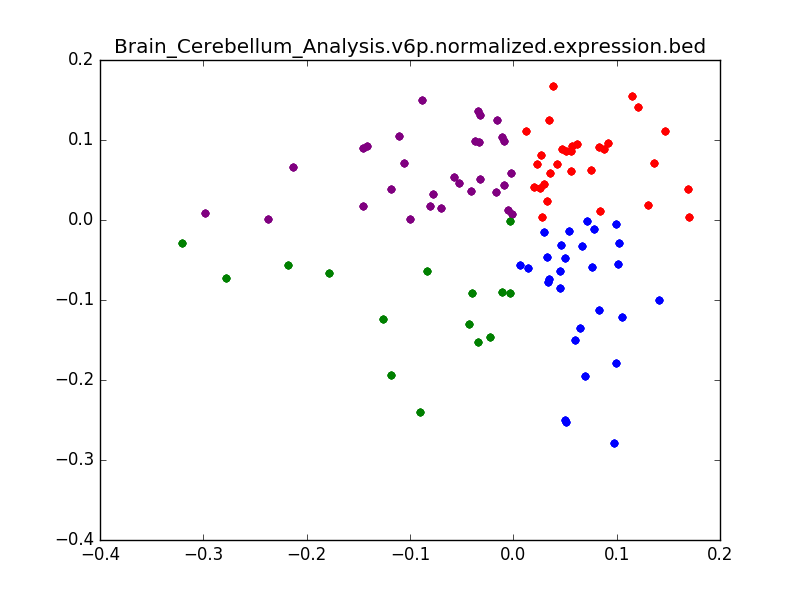
\includegraphics[scale=0.4]{Cerebellum_x_Cerebellum.png}
\end{frame}

\begin{frame} \frametitle{Comparing Tissues by Patients (Cortex)}
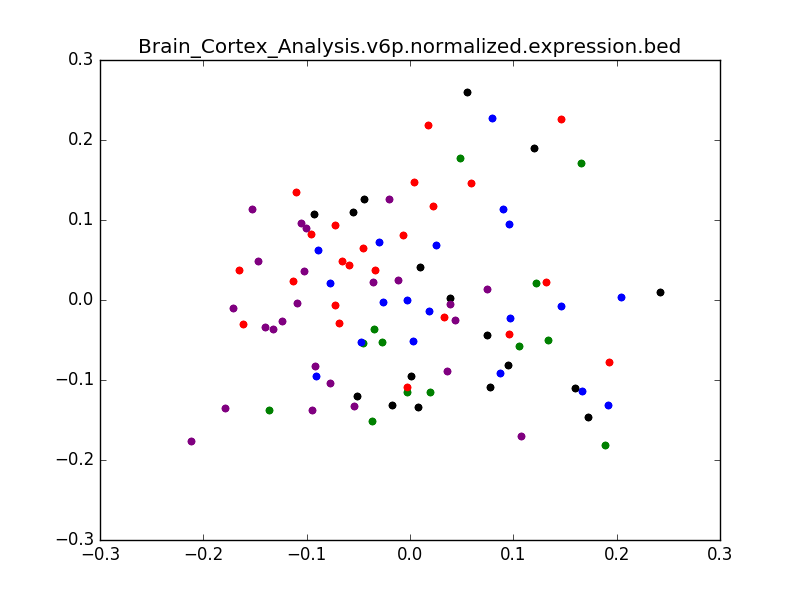
\includegraphics[scale=0.4]{Cerebellum_x_Cortex.png}
\end{frame}

\begin{frame} \frametitle{Comparing Tissues by Patients (Frontal Cortex)}
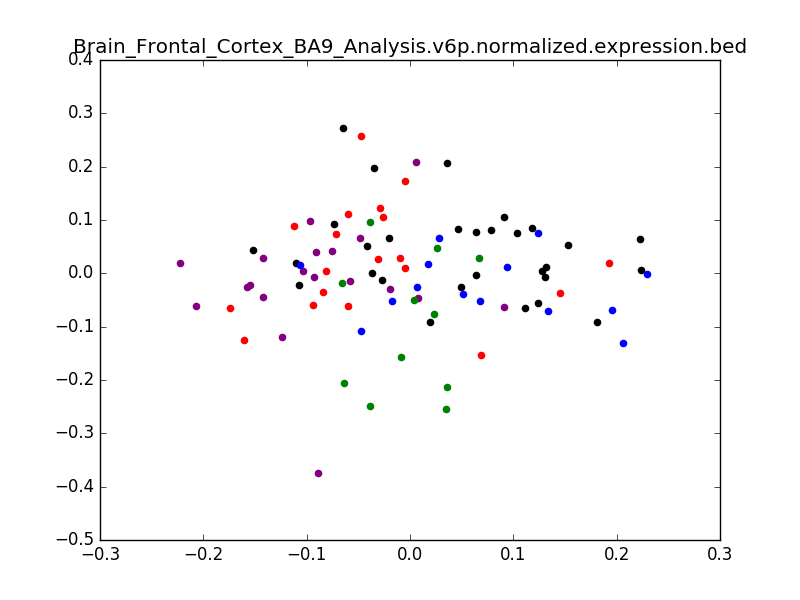
\includegraphics[scale=0.4]{Cerebellum_x_Frontal_Cortex.png}
\end{frame}

\begin{frame} \frametitle{Comparing Tissues by Patients (Lung)}
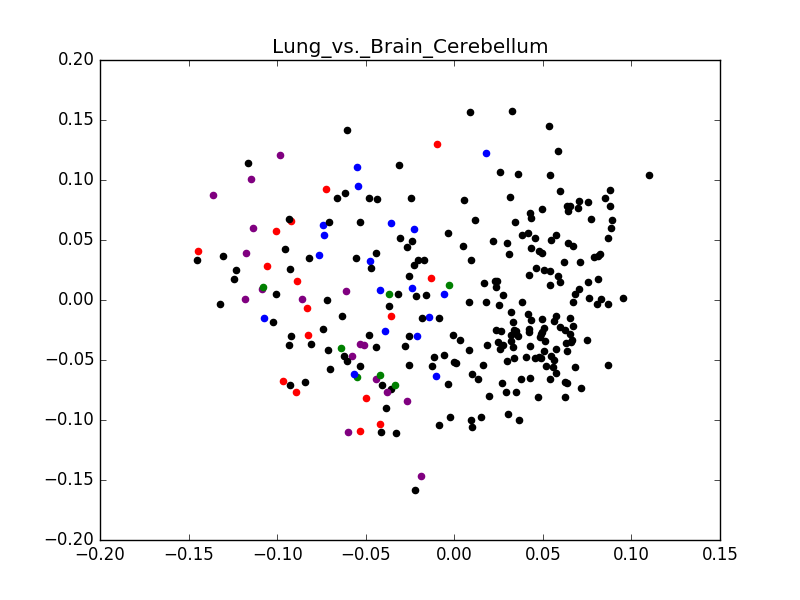
\includegraphics[scale=0.56]{Cerebellum_x_Lung.png}
\end{frame}

\begin{frame} \frametitle{Comparing Tissues by Patients (Pancreas)}
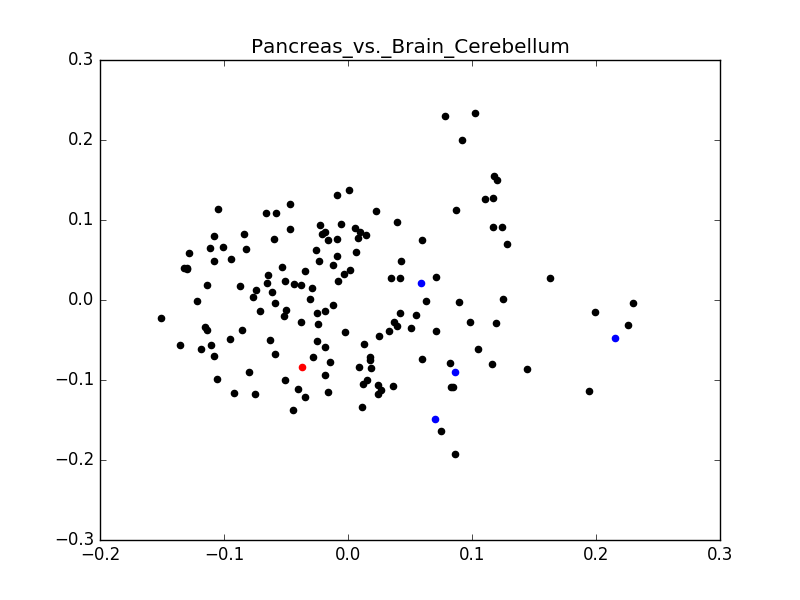
\includegraphics[scale=0.56]{Cerebellum_x_Pancreas.png}
\end{frame}


\begin{frame} \frametitle{Our algorithm}
Recall our model:
\[ Y_{iu} \sim F_i S_u + \mathcal{N}(0, \sigma^2) \]
Given either $F_i$ or $S_u$, looks like least-squares linear regression! \\

Alternate: \\
\hs{1} set $F_i \leftarrow Y_i S^T\big(SS^T)^{-1} \hs{2.8}\forall i$ \\
\hs{1} set $S_u \leftarrow \frac{1}{|I_u|}\sum_{i \in I_u} (F_i^TF_i)^{-1}F_i^T Y_{iu} \hs{1}\forall u$
\end{frame}


\begin{frame} \frametitle{BIC evaluation}
Since $F$ is derived from $S$ in closed form, so $F$ is not a free parameter. \\
$S$ has $nh$ parameters, where $n$ is the number of patients and $h$ is dimensionality of representation \\
But every solution is rotationally equivalent with solutions along $h$ degrees of freedom, leaving us $(n-1)h$ free parameters. \\
\begin{align*}
\Rightarrow \tx{BIC} &= \ln n(n-1)h -2\ln p(Y : S)
\\&= \big(\ln n\big) (n-1)h + n \ln (2\pi\sigma^2) + \frac{\tx{SSD}}{\sigma^2}
\end{align*}
\end{frame}

\begin{frame} \frametitle{BIC score across $h$ settings}
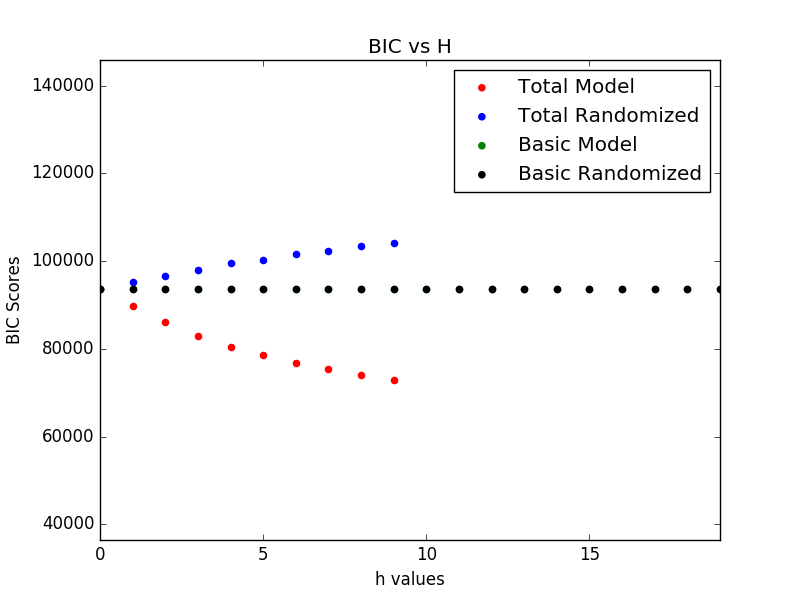
\includegraphics[scale=0.5]{BIC_Scores.png}
\end{frame}


\begin{frame} \frametitle{SSD score across $h$ settings}
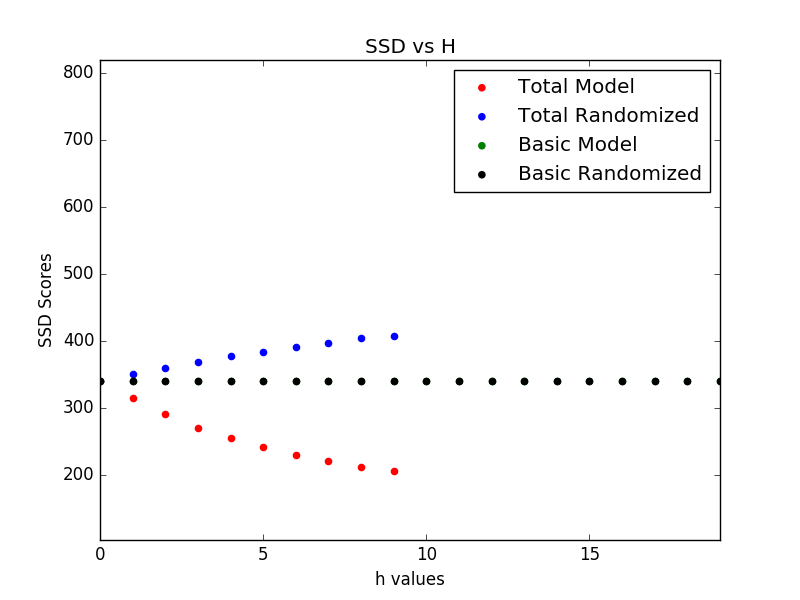
\includegraphics[scale=0.5]{SSD_Scores.png}
\end{frame}


\begin{frame} \frametitle{Applications}
{\bf Filling gaps in data}: if missing gene expression for some patient for some tissue, can just model it. \\
{\bf Comparing patients}: Can calculate cosine similarity between patients' vector representations to compare their similarity. \\
{\bf Deciding on patients}: Since all patient representations are in the same vector space, we may solve any decision problem there.
\end{frame}






























\end{document}